\documentclass[10pt, a4paper]{article}
\usepackage[utf8]{inputenc}
\usepackage[frenchb]{babel}
\usepackage[OT1]{fontenc}
\usepackage{amsfonts, amsmath, amssymb, amsthm, dsfont, amsthm}
\usepackage{a4wide}
\usepackage[dvipsnames]{xcolor}
\usepackage{tikz} 
\usetikzlibrary{arrows,positioning,shapes}

\title{\textbf{Lab Report} \\ Week of 12/01/2016}
%\author{Olivier \textsc{Mangin}}
%\date{\today}

\definecolor{main}{named}{BurntOrange}
\definecolor{second}{named}{RoyalBlue}
%\newcommand{\maincolor}{orange}
%\newcommand{\secondcolor}{orange!20}
\newcommand{\strong}[1]{\textcolor{main}{\textbf{#1}}}
\newcommand{\stronger}[1]{\textcolor{second}{\textbf{#1}}}
\newcommand{\colored}[1]{\textcolor{main}{#1}}

% Affichage du titre avec les numéro et date de la semaine
\newcommand{\titre}[2]{
\noindent
\hspace{-10pt}
\begin{tabular}{lr}
  \hspace{0.58\textwidth} & \hspace{0.4\textwidth} \\
  \strong{\huge Lab Report} & \textbf{\Large #1} \medskip \\
  \textbf{\Large Name \& Roll} & {\large #2} ~\\
\end{tabular}

\vspace{20pt}
}

% Encadré ``En bref'' réumant les avancées et problèmes de la semaine
\newenvironment{enbref}{
\noindent\fcolorbox{main}{main}{
\begin{minipage}{\textwidth}
\textcolor{white}{\textbf{\large }}
\end{minipage}
} \\

}{
\begin{center}
  \strong{ \rule[2mm]{\textwidth}{3pt} }
\end{center}
\vspace*{-20pt}
}

% Affichage d'un titre de rubrique
\newcommand{\rubrique}[1]{
  \bigskip
  \begin{center}
  \begin{minipage}{\textwidth}
    \noindent\strong{{\large #1} \\
      \rule[2mm]{\textwidth}{1pt} }
  \end{minipage}
  \end{center}
  \vspace*{-20pt}
}

% Symbole utilisé en début de ligne des éléments
\newcommand{\doublerect}{
\begin{tikzpicture}
  \fill[color=main] (0,0) rectangle (4pt,-4pt);
  \fill[color=second] (2pt,-2pt) rectangle (6pt,-6pt);
\end{tikzpicture}
}

% Affichage d'un titre d'élément
\newcommand{\element}[1]{
  \medskip
  \noindent\textcolor{second}{ \doublerect \textbf{#1}}
}

% Pour les lectures, petit raccourci pour mettre en avant le niveau
% de lecture d'un article.
\newcommand{\lu}{\strong{[Lu]} }
\newcommand{\parcouru}{\strong{[Parcouru]} }
\newcommand{\alire}{\strong{[A lire]} }
\newcommand{\presentation}{\strong{[Présentation]} }
\newcommand{\keynote}{\strong{[Keynote]} }



\usepackage[pdfauthor={Name}, pdftitle={Weekly}, pdfsubject={Week 1}, pdfkeywords={},colorlinks=true,urlcolor=black,linkcolor=black, citecolor=black]{hyperref}
\usepackage{listings}
\usepackage{subfig}
\usepackage{graphicx}
\lstset{%
language=Matlab,
frame=single,
%numbers=left,
%numberstyle=\footnotesize,
%tabsize=2,
keepspaces=true,
columns=fullflexible,
basicstyle=\ttfamily\scriptsize,
keywordstyle=\color{blue}
}


\begin{document}

\renewcommand{\labelitemi}{\textcolor{main}{\small $\blacktriangleright$}}
\renewcommand{\labelitemii}{\textcolor{second}{\scriptsize \textbullet}}

\titre{Week 8}{27/03/2017}

\begin{enbref}
\element{Title}
\begin{itemize}
\item Implement Scan converting algorithm for polygonFilling.\\
    1). OpenGL\\
    2). MatLab
\end{itemize}
\medskip
\end{enbref}

\rubrique{Procedure}
\vspace{0.5mm} \flushleft

\element {OpenGL}

\vspace{0.5mm} \flushleft
1). Choose N vertices of a polygon and apply the algorithm  described below :
\begin{itemize}
\item Create a C file and name it as \textit{polygonFilling.c}.
\item Following is the final code :
\begin{lstlisting}
#include <GL/glut.h>
#include <stdio.h>
#include <stdlib.h>

int point;
int points[99999];

int cmpfunc (const void * a, const void * b)
{
        return ( (*(float*)a > *(float*)b ) ? 1 : 0);
}

int update (int a,int b)
{
	if(a-b>0)
        {        // going up
		return 1;
	}
	if(a-b<0)
        {        // going down
		return -1;
	}
	if(a-b==0)
        {       // horizontal
		return 0;
	}
}

float find_inter(int x,int y,int a,int b,int line)
{
	printf("Finding intersection : %d %d %d %d %d ",x,y,a,b,line);
	float result;
	int ymin;
	int ymax;
	int xmin;
	int xmax;
	if(y<b)
        {
		ymin=y;
		ymax=b;
	}
	else
        {
		ymin=b;
		ymax=y;
	}
	if(x<a)
        {
		xmin=x;
		xmax=a;
	}
	else
        {
		xmin=a;
		xmax=x;
	}
	if(a-x==0)
        {
		if(line<ymin || line>ymax)
                {
			result=-999999;
		}
		else
                {
			result=x;
		}
	}
	else if(b-y==0)
        {
		result= -999999;
		printf("parallel ");
	}
	else
        {
		if(line<ymin || line >ymax)
                {
			result=-999999;
		}
		else
                {
			result = x+((line-y)/((b-y)/(float)(a-x)));
		}
	}
	printf("%f \n",result);
	return result;
}
void display(void)
{
	int i=0;
	int j=0;
	int k=0;
	int ymax=-999999999,ymin=999999999;
	for(i=0;i<2*point;i+=2)
        {
		if(points[i+1]>ymax)
                {
			ymax=points[i+1];
		}
		if(points[i+1]<ymin)
                {
			ymin=points[i+1];
		}
	}
	float final_points[99999];
	int tot=0;
	for(i=ymin;i<ymax+1;i++)
        {
		float inter_points[99999];
		int count=0;
		int flag=0;
		float prev_inter_point=-999999;
		for(j=0;j<2*(point-1);j+=2)
                {
			float inter_point = find_inter(points[j],points[j+1],points[j+2],points[j+3],i);
			if(inter_point==-999999)
                        { // no intersection point
				flag = update(points[j+3],points[j+1]);
				prev_inter_point=inter_point;
				continue;
			}
			if(points[j+3]-points[j+1]>0)
                        { // going up
				if(flag==1 && prev_inter_point==inter_point)
                                {
					flag = update(points[j+3],points[j+1]);
					prev_inter_point=inter_point;
					continue;
				}
			}
			else if(points[j+3]-points[j+1]<0)
                        { // going down
				if(flag==-1 && prev_inter_point==inter_point)
                                {
					flag = update(points[j+3],points[j+1]);
					prev_inter_point=inter_point;
					continue;
				}
			}
			inter_points[count]= inter_point;
			flag = update(points[j+3],points[j+1]);
			prev_inter_point=inter_point;
			count++;
		}
		float inter_point = find_inter(points[2*point-2],points[2*point-1],points[0],points[1],i);
		if(inter_point!=-999999)
                {
			if(points[1]-points[2*point-1]>0)
                        { // going up
				if(flag!=1 || prev_inter_point!=inter_point)
                                {
					inter_points[count]=inter_point;
					count++;
				}
			}
			else if(points[1]-points[2*point-1]<0)
                        { // going down
				if(flag!=-1 || prev_inter_point!=inter_point)
                                {
					inter_points[count]=inter_point;
					count++;
				}
			}
			else
                        { // horizontal
				inter_points[count]=inter_point;
				count++;
			}
		}
		qsort(inter_points, count, sizeof(float), cmpfunc);
		printf("Intersection co-ordinates\n");
		for(k=0;k<count;k=k+1)
                {
			printf("%f %d\n",inter_points[k],i);
		}
		printf("All points\n");
		for(k=0;k<count;k=k+2)
                {
			float l=0;
			if(k>=count-1)
                        {
				break;
			}
			for(l=inter_points[k];l<=inter_points[k+1];l=l+1)
                        {
				final_points[tot]=l;
				tot++;
				final_points[tot]=i;
				tot++;
				printf("%f %d\n",l,i);
			}
		}
	}

	printf("Plotting filled points\n");
	       glClear(GL_COLOR_BUFFER_BIT);
	                glPointSize(1.0);
                        glBegin(GL_LINES);
                                glColor3f(0.0,0.0,0.0);
                                glVertex2d(-300,0);
                        	glVertex2d(300,0);
                        	glVertex2d(0,300);
                        	glVertex2d(0,-300);
                                glColor3f(0.0,1.0,0.0);
	                glEnd();

        glBegin(GL_POINTS);
	       for(i=0;i<tot;i+=2)
                {
		        printf("%f %f\n",final_points[i],final_points[i+1]);
		        glVertex2f(final_points[i],final_points[i+1]);
	        }
	glEnd();
	glFlush();
}
void Init()
{
	/* Set clear color to white */
	glClearColor(1.0,1.0,1.0,1);
	/* Set fill color to black */
	glColor3f(0.0,0.0,0.0);
	gluOrtho2D(-300 , 300 , -300 , 300);
}
int main (int argc, char **argv){
	int i;
	printf("Enter the no. of points in the polygon : ");
	scanf("%i",&point);
	for(i=0;i<2*point;i+=2)
        {
		printf("Enter the co-ordinate of %dth point     : ",(i/2)+1);
		scanf("%i%i",&points[i],&points[i+1]);
	}
	/* Initialise GLUT library */
	glutInit(&argc,argv);
	/* Set the initial display mode */
	glutInitDisplayMode(GLUT_SINGLE | GLUT_RGB);
	/* Set the initial window position and size */
	glutInitWindowPosition(0,0);
	glutInitWindowSize(600,600);
	/* Create the window with title "DDA_Line" */
	glutCreateWindow("Polygon filling algorithm");
	/* Initialize drawing colors */
	Init();
	/* Call the displaying function */
	glutDisplayFunc(display);
	/* Keep displaying untill the program is closed */
	glutMainLoop();
	return 0;
}

\end{lstlisting}

\vspace{0.5mm}

\item Compile and run the executable file in terminal by typing in the following commands : \\

\vspace{0.5mm} \flushleft

\textit{(a)\hspace{2mm} gcc polygonFilling.c -lGL -lGLU -lglut -ll} \\
\textit{(b)\hspace{2mm} ./a.out}
\vspace*{1\baselineskip}
\end{itemize}

\element {MatLab}\\

1). Choose N Vertices of a polygon and  apply the algorithm described below :

\begin{itemize}

\item Open a new matlab script and define a function polygonFilling().
\item Following is the final code.
\begin{lstlisting}

clc
clear

function func = update(a,b)
	if(a-b>0)
		func=1;
	elseif(a-b<0)
		func=-1;
	else
		func=0;
	end
end

function func = find_inter(x,y,a,b,line)
	result=0;
	ymax = 0;
	ymin = 0;
	xmax = 0;
	xmin = 0;
	if(x>a)
		xmin=a;
		xmax=x;
	else
		xmin=x;
		xmax=a;
	end
	if(y>b)
		ymin=b;
		ymax=y;
	else
		ymin=y;
		ymax=b;
	end
	if(b==y)
		result=-999999;
	elseif(a==x)
		if(line>=ymin && line<=ymax)
	  		result = x;
		else
	  		result=-999999;
	  end
	else
		if(line<ymin || line>ymax)
	  		result=-999999;
		else
	  		result= x+((line-y)/((b-y)/(a-x)));
	  end
	end
	func = result;
end

point = input("Enter the no. of points in polygon:	");
x_vals = [];
y_vals = [];
for i = 1:point
	x = input("Enter the x co-ordinate of point:	");
	y = input("Enter the y co-ordinate of point:	");
	x_vals(i)=x;
  	y_vals(i)=y;
end
ymin=y_vals(1);
ymax=y_vals(1);
for i= 2:point
	if(y_vals(i)>ymax)
		ymax=y_vals(i);
	elseif(y_vals(i)<ymin)
		ymin=y_vals(i);
	end
end
ymin;
ymax;
final_points_x = [];
tot_x = 1;
final_points_y = [];
tot_y = 1;
for i = ymin:ymax
	i
	flag = 0;
	count = 1;
	prev_inter_point = -999999;
	inter_points = [];
	for j = 1:point-1
		inter_point = find_inter(x_vals(j),y_vals(j),x_vals(j+1),y_vals(j+1),i);
		if(inter_point==-999999)
			flag=update(y_vals(j+1),y_vals(j));
			prev_inter_point=inter_point;
			continue
		end
		if(y_vals(j+1)-y_vals(j)>0)
			if(flag==1 && prev_inter_point==inter_point)
				flag=update(y_vals(j+1),y_vals(j));
				prev_inter_point=inter_point;
				continue
			end
		elseif(y_vals(j+1)-y_vals(j)<0)
			if(flag==-1 && prev_inter_point==inter_point)
				flag=update(y_vals(j+1),y_vals(j));
				prev_inter_point=inter_point;
				continue
			end
		end
		inter_points(count) = inter_point;
		flag = update(y_vals(j+1),y_vals(j));
		prev_inter_point=inter_point;
		count=count+1;
	end
	inter_point = find_inter(x_vals(point),y_vals(point),x_vals(1),y_vals(1),i);
	if(inter_point!=-999999)
		if(y_vals(1)-y_vals(point)>0)
			if(flag!=1 || prev_inter_point!=inter_point)
				inter_points(count) = inter_points;
				count=count+1;
			end
		elseif(y_vals(1)-y_vals(point)<0)
			if(flag!=-1 || prev_inter_point!=inter_point)
				inter_points(count) = inter_point;
				count=count+1;
			end
		else
			inter_points(count) = inter_point;
			count=count+1;
		end
	end
	inter_points;
	inter_points=sort(inter_points);
	for j = 1:2:count-2
    a=inter_points(j);
    b=inter_points(j+1);
		for k = a:b
			final_points_x(tot_x)= k;
			final_points_y(tot_y)= i;
			tot_x=tot_x+1;
			tot_y=tot_y+1;
		end
	end
end
axis_x= [-300,300];
axis_y= [0,0];
line(axis_x,axis_y,'Color',[0.0,1.0,0.0],'LineWidth',2);
axis_y= [-300,300];
axis_x= [0,0];
line(axis_x,axis_y,'Color',[0.0,1.0,0.0],'LineWidth',2);
hold on
scatter(final_points_x,final_points_y)
axis([-300 300 -300 300]);
xlabel('X-Axis');
ylabel('Y-Axis');
title('Polygon filling algorithm');

\end{lstlisting}
\end{itemize}
\rubrique{Output}
\begin{figure}[ht!]
\centering
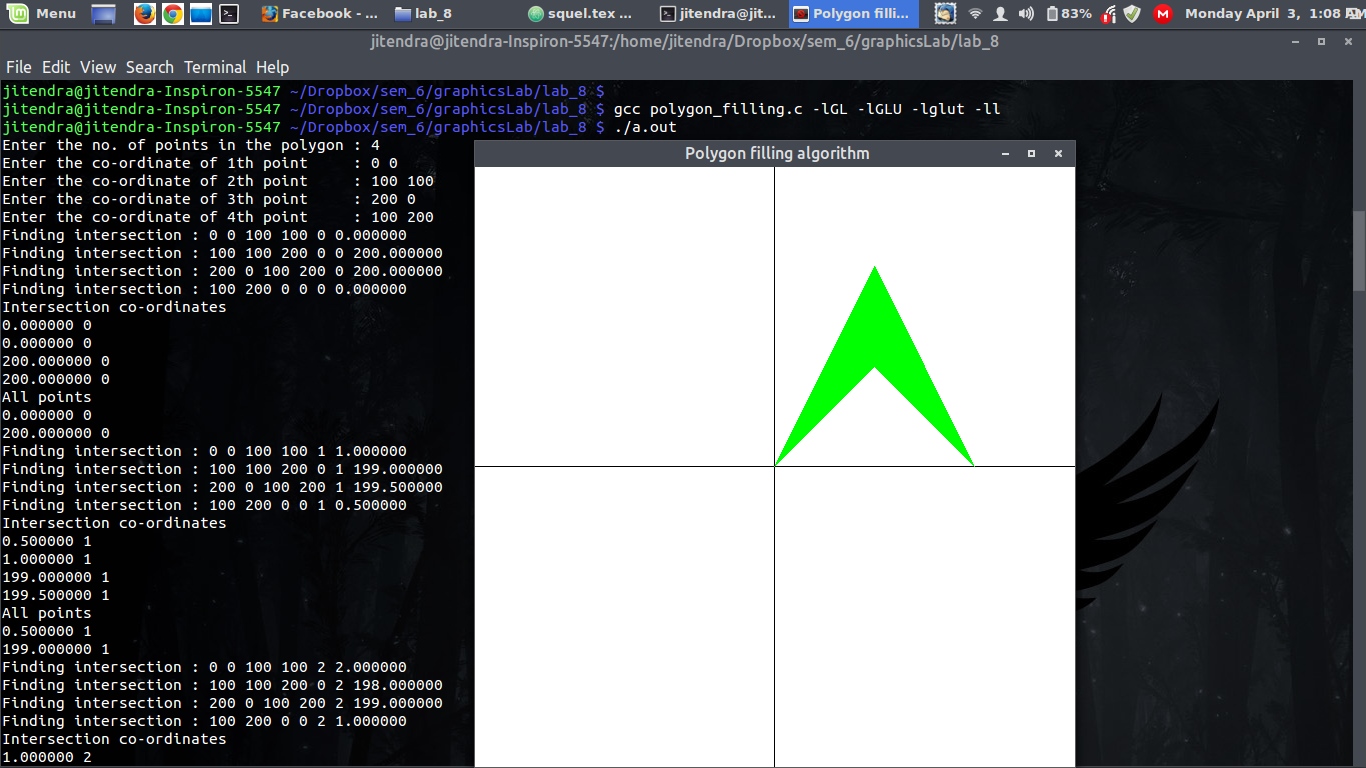
\includegraphics[width=150mm, height=100mm]{openGL.png}
\caption{openGL output \label{overflow}}
\end{figure}
\begin{figure}[ht!]
\centering
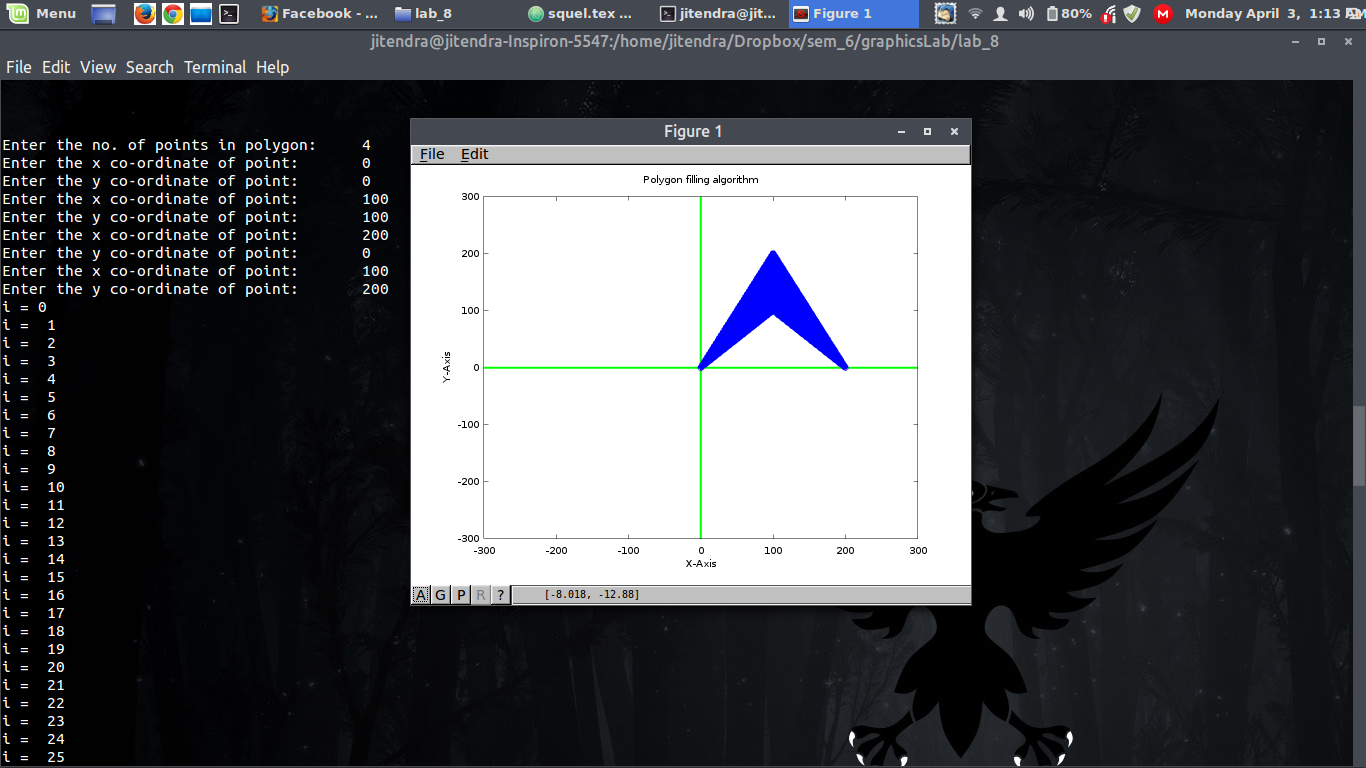
\includegraphics[width=150mm, height=100mm]{matlab.png}
\caption{matlab output \label{overflow}}
\end{figure}
\end{document}
